
\documentclass{article}

\usepackage[utf8]{inputenc}
%\usepackage[latin1]{inputenc}
\usepackage[T1]{fontenc}

\usepackage[french]{babel}
\usepackage{amsmath}
\usepackage{amsfonts}
\usepackage{amssymb}
\usepackage{graphicx}
\usepackage{hyperref}
\usepackage{psfrag}
\usepackage{subfigure}
\usepackage{xspace}
\usepackage{pxfonts}
\usepackage{listings}
\usepackage[myheadings]{fullpage}
\usepackage{url}
\usepackage{verbatim}
\usepackage{makeidx}
\usepackage{cclicenses}
\usepackage{fancyhdr}
\usepackage{color}
\usepackage{tikz}
\usepackage{lastpage}
\usetikzlibrary{shadows}
\usepackage{titlesec}


\author{Jonathan Ferreira}
\title{WHILE - Un interpréteur visuel pour les langages WHILE(A)\\
\large Guide de l'utilisateur}
\date{Septembre 2020}


\begin{document}

\maketitle

\clearpage
\newpage

\tableofcontents


\clearpage
\newpage



%\section*{Préliminaire}

%Sed ut perspiciatis unde omnis iste natus error sit voluptatem accusantium doloremque laudantium, totam rem aperiam, eaque ipsa quae ab illo inventore veritatis et quasi architecto beatae vitae dicta sunt explicabo. Nemo enim ipsam voluptatem quia voluptas sit aspernatur aut odit aut fugit, sed quia consequuntur magni dolores eos qui ratione voluptatem sequi nesciunt. Neque porro quisquam est, qui dolorem ipsum quia dolor sit amet, consectetur, adipisci velit, sed quia non numquam eius modi tempora incidunt ut labore et dolore magnam aliquam quaerat voluptatem. Ut enim ad minima veniam, quis nostrum exercitationem ullam corporis suscipit laboriosam, nisi ut aliquid ex ea commodi consequatur? Quis autem vel eum iure reprehenderit qui in ea voluptate velit esse quam nihil molestiae consequatur, vel illum qui dolorem eum fugiat quo voluptas nulla pariatur?

%\clearpage
%\newpage

\section{Introduction}
\label{sec:introduction}

Ce guide explique l'utilisation de l'interpréteur visuel (ci-après nommé "logiciel" ou "application") pour la famille de langages WHILE(A) (ci après nommé "langage WHILE" ou "WHILE").

\subsection{Prérequis}

Comme l'utilisation de WHILE est une partie intégrante du logiciel, il est nécessaire de connaître la syntaxe du langage WHILE afin de pouvoir utiliser le logiciel.



\section{Lancement du logiciel}


\subsection{Lancement en ligne}
\label{sec:lancement}
Le logiciel consiste en une simple page web. En tant que tel, le lancement de celui-ci est extrêmement simple. Un accès à Internet est requis. Il suffit à l'aide d'un navigateur web moderne (Firefox, Chrome, Edge, etc.) d'aller à l'URL \url{https://alphajon.github.io/WhileInterpret/} et le logiciel se chargera directement dans le navigateur. Vous verrez ainsi quelque chose ressemblant à la figure \ref{fig:cap1} suivante

\begin{figure}[h]
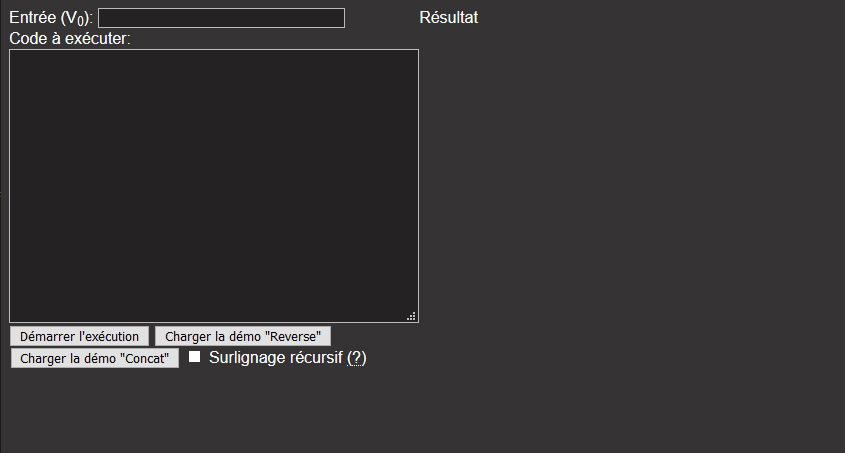
\includegraphics[width=\textwidth]{img/Capture1.PNG}
\caption{Logiciel WHILE}
\label{fig:cap1}
\end{figure}

\subsection{Téléchargement pour un usage hors ligne}

Il est possible de télécharger le logiciel pour un usage ultérieur en local sans accès à Internet. Pour télécharger le logiciel, ouvrez l'application en suivant les instructions de la section \ref{sec:lancement}, puis effectuez un clic droit sur une section vide de la page web de l'application. Sélectionnez ensuite "Enregistrer sous..." puis choisissez un dossier de destination pour le téléchargement.

Une fois l'application téléchargée, il suffit d'ouvrir le fichier nouvellement créé avec un double-clic, ce qui devrait charger automatiquement l'application dans un navigateur web.

Cette méthode n'est cependant pas recommandée, car les mises à jour pour le logiciel ne seront pas disponibles via la version hors ligne.


\section{Utilisation du logiciel}

Le logiciel est conçu de manière à être très simple d'utilisation. En effet, il ne comporte qu'une poignée de boutons, et un faible nombre de champs texte.

Pour pouvoir lancer l'interpréteur, l'application a besoin de connaître le programme WHILE à exécuter, ainsi que la valeur d'entrée $V_0$ qui doit être assignée à ce programme. Des programmes exemples sont cependant fournis via les différents boutons \og Lancer la démo \fg{} présents sur la partie inférieure de l'application, qui pré-remplissent les champs requis.

\subsection{Entrée d'un programme WHILE}

Le programme WHILE que vous souhaitez exécuter doit être entré dans le champ nommé \og Code à exécuter \fg{} présent dans l'application. Le programme doit être syntaxiquement valide. Si le programme n'est pas syntaxiquement valide, l'interpréteur ne se lancera pas, et une erreur sera affichée à l'écran, comme sur la figure \ref{fig:cap2}.

\begin{figure}[h]
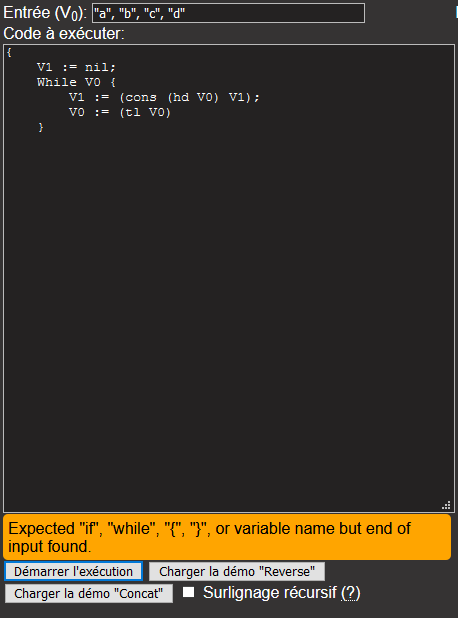
\includegraphics[width=\textwidth]{img/Capture2.PNG}
\caption{Exemple d'erreur}
\label{fig:cap2}
\end{figure}

\subsection{Entrée de la valeur de départ V0}

La valeur d'entrée doit être indiquée dans le champ nommé \og Entrée ($V_0$) \fg{}. Afin d'éviter un usage excessif d'imbrications, de parenthèses et d'expressions \og cons \fg{}, une syntaxe spécifique pour l'entrée est fournie.

Les atomes doivent être entourées de guillemets doubles. Ceci permettra de différencier par exemple entre $"nil"$ et la valeur spéciale $nil$. Pour indiquer des couples, les virgules $,$ et les points-virgules $;$ peuvent être utilisés pour séparer des valeurs (des atomes ou d'autres couples), et ont un comportement différent:
\newline

La virgule sépare des valeurs successives de telle sorte à ce que l'entrée $("t1", "t2", "t3", "t4")$ représente l'arbre $(t1, (t2, (t3, (t4, nil))))$
Le point-virgule sépare deux valeurs, et représente directement un couple. $("t1"; "t2")$ représente donc $(t1, t2)$. $("t1", "t2")$ aurait à la place représenté $(t1, (t2, nil)$. Il ne peut y avoir qu'une seule valeur (atome ou couple) du côté droit du point-virgule.
\newline

Il est donc aussi possible d'écrire $("t1", "t2", "t3"; "t4")$, avec un point-virgule entre les deux derniers éléments d'un groupe de valeurs \textbf{uniquement}, qui permet de placer ces deux éléments en fin d'arbre dans le même couple. Ainsi, $("t1", "t2", "t3"; "t4")$ représente l'arbre $(t1, (t2, (t3, t4)))$, mais $("t1", "t2"; "t3", "t4"; "t5")$ est une syntaxe invalide. Pour corriger cela, on peut utiliser $("t1", ("t2"; "t3"), "t4"; "t5")$ si le point-virgule ne doit s'appliquer que sur l'élément suivant,  ou $("t1", "t2"; ("t3", "t4"; "t5"))$ si le point-virgule doit s'appliquer sur le reste des éléments
\newline

Comme pour l'entrée du programme, si l'entrée de la valeur $V_0$ n'est pas syntaxiquement valide, l'interpréteur ne se lancera pas, et une erreur sera affichée à l'écran.


\subsection{Exécution du programme}

Une fois que la valeur d'entrée et le programme donnés au logiciel sont entrés, et si tous deux sont valides, le logiciel débutera l'interprétation du programme. L'application ressemblera alors à la figure \ref{fig:cap3}.

\begin{figure}[h]
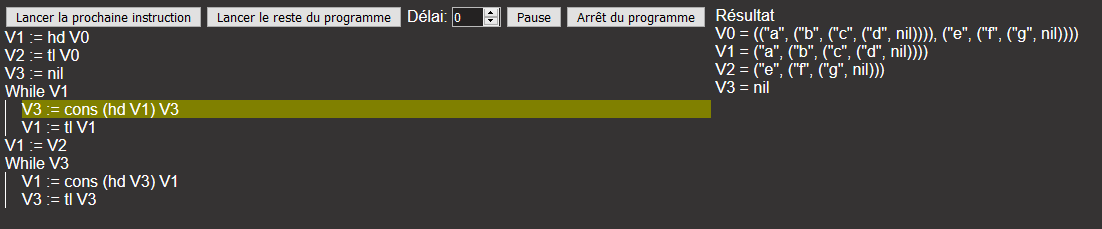
\includegraphics[width=\textwidth]{img/Capture3.PNG}
\caption{Interprétation d'un programme en cours}
\label{fig:cap3}
\end{figure}

Le programme en cours d'exécution est représenté, avec une mise en surbrillance de la prochaine ligne à exécuter sur la moitié gauche de l'application, et le contenu de la mémoire du programme en cours est affichée sur la moitié droite de l'application. Vous pouvez alors interagir avec le programme via les boutons proposés. Si aucune ligne du programme n'est mise en surbrillance, cela signifie que le programme a terminé son exécution.

\subsubsection{Lancer la prochaine instruction}
Exécute une seule instruction (celle mise en surbrillance par l'application). L'instruction suivante (s'il y en a une) est alors mise en surbrillance, indiquant l'instruction qui sera exécutée en appuyant sur le bouton une fois de plus.

\subsubsection{Lancer le reste du programme}
Ordonne au logiciel de lancer le reste du programme, à hauteur d'une instruction toutes les $X$ secondes, où $X$ représente la valeur qui était présente dans le champ "Délai" au moment de l'appui du bouton. Une valeur de 0 lance instantanément tout le reste du programme en cours jusqu'à la fin. Le bouton "Pause" interrompt l'exécution automatique.

\subsubsection{Arrêt du programme}
Interrompt le programme en cours, et retourne sur le formulaire d'entrée du programme de la figure \ref{fig:cap1}.

\end{document}
